\documentclass[a4paper, 12pt]{article}

\usepackage{graphicx}
\usepackage{longtable}
\graphicspath{ {images/} }

\newcommand{\templates}{../../template}
\usepackage[a4paper, margin=2.5cm]{geometry}

\usepackage{enumitem}
\setlist[itemize]{noitemsep}
\setlist[enumerate]{noitemsep}

\let\oldpar\paragraph
\renewcommand{\paragraph}[1]{\oldpar{#1\\}\noindent}
\usepackage{graphicx}
\usepackage{hyperref}
\usepackage{makecell}

\newcommand{\settitolo}[1]{\newcommand{\titolo}{#1\\}}
\newcommand{\setprogetto}[1]{\newcommand{\progetto}{#1\\}}
\newcommand{\setcommittenti}[1]{\newcommand{\committenti}{#1\\}}
\newcommand{\setredattori}[1]{\newcommand{\redattori}{#1\\}}
\newcommand{\setrevisori}[1]{\newcommand{\revisori}{#1\\}}
\newcommand{\setresponsabili}[1]{\newcommand{\responsabili}{#1\\}}
\newcommand{\setversione}[1]{
	\ifdefined\versione\renewcommand{\versione}{#1\\}
	\else\newcommand{\versione}{#1\\}\fi
}
\newcommand{\setdestuso}[1]{\newcommand{\uso}{#1\\}}
\newcommand{\setdescrizione}[1]{\newcommand{\descrizione}{#1\\}}

\newcommand{\makefrontpage}{
	\begin{titlepage}
		\begin{center}

		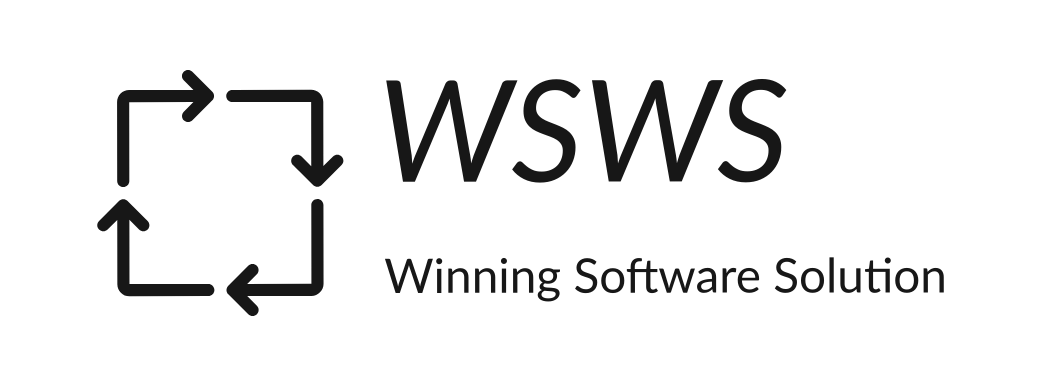
\includegraphics[width=0.4\textwidth]{../../template/WSWS-logos_transparent_crop}\\

		{\Large Winning Software Solution}\\[6pt]
		\href{mailto://winningsoftwaresolution@gmail.com}{winningsoftwaresolution@gmail.com}\\
		
		\ifdefined\progetto
		\vspace{1cm}
		{\Large\progetto}
		{\large\committenti}
		\else\fi
		
		\vspace{1.5cm}
		{\LARGE\titolo}
		
		\vfill
		
		\begin{tabular}{r | l}
		\multicolumn{2}{c}{\textit{Informazioni}}\\
		\hline
		
		\ifdefined\redattori
			\textit{Redattori} &
			\makecell[l]{\redattori}\\
		\else\fi
		\ifdefined\revisori
			\textit{Revisori} &
			\makecell[l]{\revisori}\\
		\else\fi
		\ifdefined\responsabili
			\textit{Respondabili} &
			\makecell[l]{\responsabili}\\
		\else\fi
		
		\ifdefined\versione
			\textit{Versione} & \versione
		\else\fi
		
		\textit{Uso} & \uso
		
		\end{tabular}
		
		\vspace{2cm}
		
		\ifdefined\descrizione
		Descrizione
		\vspace{6pt}
		\hrule
		\descrizione
		\else\fi
		\end{center}
	\end{titlepage}
}
\usepackage{hyperref}
\usepackage{array}
\usepackage{tabularx}

\def\vers#1-#2-#3-#4-#5\\{#1&#2&#3&#4&#5\\\hline}

\newcommand{\addversione}[5]{
	\ifdefined\versioni
		\let\old\versioni
		\renewcommand{\versioni}{#1&#2&#3&#4&#5\\\hline\old}
	\else
		\newcommand{\versioni}{#1&#2&#3&#4&#5\\\hline}
	\fi
}

\newcommand{\setversioni}[1]{\newcommand{\versioni}{#1}}

\newcommand{\makeversioni}{
	\begin{center}
		\begin{tabularx}{\textwidth}{|c|c|c|c|X|}
		\hline
		\textbf{Versione} & \textbf{Data} & \textbf{Persona} & \textbf{Attivtà} & \textbf{Descrizione} \\
		\hline
		\versioni
		\end{tabularx}
	\end{center}
	\clearpage
}

\settitolo{Analisi dei requisiti}
\setprogetto{ShopChain}
\setcommittenti{SyncLab}
\setredattori{Giovanni Cocco}
\setrevisori{Federico Marchi}
\setresponsabili{Giovanni Cocco}
\setdestuso{esterno}
\setdescrizione{
Architettura del progetto
}

\addversione{0.0.0}{23/2/2022}{Raffaele Oliviero}{Redazione}{Strutturazione del documento}


\begin{document}

\makefrontpage

\makeversioni

\section{Introduzone}
\subsection{Scopo del documento}
Il documento illustra le scelte architetturali e illustra l'architettura tramite diagrammi delle classi e di sequenza.

\section{Tecnologie/Linguaggi/Librerie}
\subsection{Python}
\begin{itemize}
\item \textbf{Versione:}
\item \textbf{Documentazione:}
\end{itemize}

\subsection{Typescript}
\begin{itemize}
\item \textbf{Versione:}
\item \textbf{Documentazione:}
\end{itemize}

\subsection{Moralis}
\begin{itemize}
\item \textbf{Versione:}
\item \textbf{Documentazione:}
\end{itemize}

\subsection{Whatever}
\begin{itemize}
\item \textbf{Versione:}
\item \textbf{Documentazione:}
\end{itemize}

\section{Architettura}
Il progetto si compone di 4 macro parti:
\begin{itemize}
\item Server
\item Smart contract
\item Web app
\item Script di messa in vendita
\end{itemize}
\subsection{Server}
\subsubsection{Diagramma delle classi}
[grafico]
\paragraph{Commenti}
\subsubsection{Pattern architetturale adottato}
\paragraph{Descrizione}
\paragraph{Motivazioni}

\subsection{Smart contract}
\subsubsection{Diagramma delle classi}
[Qua si può lasciare un commento su eventuali convenzioni adottate, tipo come identificare gli external di solidity]
[grafico]
\paragraph{Commenti}
\subsubsection{Pattern architetturale adottato}
\paragraph{Descrizione}
\paragraph{Motivazioni}

\subsection{Web app}
\subsubsection{Diagramma delle classi}
[grafico]
\paragraph{Commenti}
\subsubsection{Pattern architetturale adottato}
\paragraph{Descrizione}
\paragraph{Motivazioni}

\subsection{Script di messa in vendita}
\subsubsection{Diagramma delle classi}
[grafico]
\paragraph{Commenti}
\subsubsection{Pattern architetturale adottato}
\paragraph{Descrizione}
\paragraph{Motivazioni}


\clearpage

\section{Pattern Architetturali}
In alternativa, se un pattern è utilizzato più volte o è particolarmente complicato si può fare una sezione apposita in cui reindirizzare le sottosezioni all'interno dell'architettura. (Ovviamente eviterei di mischiare le due modalità, cioè all'interno della sezione architettura, o mettiamo tutto quello che riguarda i design pattern, o mettiamo le motivazioni per cui abbiamo adottato un certo pattern e poi mettiamo un riferimento a questa sezione)
\subsection{Pattern Architetturale 1}
[descrizione]



\clearpage

\section{Diagrammi di sequenza}
\subsection{Server}
[grafico]
\paragraph{Commenti}

\subsection{Ascolto eventi del contratto}
[grafico]
\paragraph{Commenti}

\subsection{Inizializzazione server web}
[grafico]
\paragraph{Commenti}

\subsection{Nuovo oggetto in vendita}
[grafico]
\paragraph{Commenti}

\subsection{Nuova transazione}
[grafico]
\paragraph{Commenti}

\subsection{Cambio di stato di una transazione}
[grafico]
\paragraph{Commenti}

\subsection{Home page}
[grafico]
\paragraph{Commenti}

\subsection{Landing page di vendita}
[grafico]
\paragraph{Commenti}

\subsection{Dettagli transazione}
[grafico]
\paragraph{Commenti}

\subsection{Pagina di sblocco fondi (arrivo del pacco)}
[grafico]
\paragraph{Commenti}

\subsection{Lista oggetti venduti}
[grafico]
\paragraph{Commenti}

\subsection{Lista oggetti comprati}
[grafico]
\paragraph{Commenti}

\subsection{Manuale utente}
[grafico]
\paragraph{Commenti}

\end{document}